% Chapter Template

\chapter{Event selection and background estimation} % Main chapter title

\label{Chapter6} % Change X to a consecutive number; for referencing this chapter elsewhere, use \ref{ChapterX}

\lhead{Chapter 6. \emph{Event selection and background estimation}} % Change X to a consecutive number; this is for the header on each page - perhaps a shortened title



\section{Data and Monte Carlo samples}

%----------------------------------------------------------------------------------------
%	SECTION 1
%----------------------------------------------------------------------------------------

\section{Event selection}
\label{sec:selection}
Signal events are characterized by presence of a W boson and two jets which have been tagged as coming from b quarks.
Candidates for a W boson are identified as isolated muons or electron and significant missing energy.
Jets are identified as particle flow objects clustered with anti-$k_T$ algorithm with a cone size of $0.5$.
Standard jet energy corrections and resolution smearing procedures prescribed by the Jet POG are applied.
Combined secondary vertex (CSV) algorithm is then used to identify jets arising from fragmentation and hadronization of b-quarks.
This algorithm combines in an optimal way information about track impact parameters and identified secondary vertices
within the jet even when full vertex information is not available.
Isolated leptons not arising from W decays are not expected, and additional jet activity is minimal.




%----------------------------------------------------------------------------------------
%	SECTION 2
%----------------------------------------------------------------------------------------

\section{Background estimation}

After applying all selection cuts described in the previous section, major backgrounds that remain are top quark, Z+jets, W+jets, diboson and QCD background. Each of the background contributions is described in detail below. 


\subsection{Top quark background}

Production of $t\bar{t}$ pairs and single top represent a challenging background at the LHC because of their relatively large production cross sections. $t\bar{t}$ events are largely reduced by requiring an additional jet veto. Single top events are more difficult to reject relative to signal using just topological cuts, but production cross-section is smaller resulting in a smaller contribution in the final distributions.
With very large contribution of the $t\bar{t}$ background, a test of the normalization was performed. A separate control region was created which was defined to be same as signal region, but requiring additional jet activity. This results in a $t\bar{t}$ enriched sample where it is visible that the shape of the distribution is well described in the simulation, but the overall normalization is too small. 

\subsection{Z+jets}

The contribution from the events where Z boson is produced in association with two b jets is largely suppressed by requiring only one lepton in the event. However, it can happen that one of the leptons from Z decay escapes the detection or is missidentified which possibly causes significant missing energy. Such events are than passing all selection criteria and have to be taken into account in the final cross section measurement. 

\subsection{W+light jets and W+charm}



\subsection{QCD}

QCD background arises from QCD events containing soft leptons. An example of such event is shown in the left part of figure \ref{fig:QCD}. This is one of the more challenging backgrounds as it is difficult to simulate significant amount of such events without restrictions. Therefore, the contribution of QCD events in the signal region is determined from data. The illustration of the method is shown in the right part of figure \ref{fig:QCD}. Two uncorrelated variables are chosen, in this case transverse mass and lepton isolation. Signal region is shown in the region A. Control sample dominated by QCD events is created by inverting the lepton isolation cut to $iso>0.2$($0.15$) for muons(electrons) which is shown as region C. The rest of the selection criteria in the control sample is the same as in signal region. It is assumed that the QCD distribution has the same shape in regions A and C. The obtained sample is relatively clean, the shape of the distribution is determined by subtracting the simulation events that pass the selection. Normalization of the distribution is determined form the $M_T$ region below 30 GeV. Fake rate is determined from regions B and D by subtracting simulation number of simulated events that pass the cuts from the number of data events. The final normalization is than expressed as:
\begin{equation}
QCD^A=\frac{N^B_{data}-N^B_{MC}}{N^D_{data}-N^D_{MC}}\times QCD^{C}_{data}
\end{equation}       
where $N^B_{data}$ and $N^D_{data}$ are the number of data events in data in regions B and D respectively, and $N^C_{MC}$ and $N^D_{MC}$ are the number of MC events in regions B and D respectively. The signal region before and after the QCD contribution determination is shown in figure \ref{fig:QCD_dist}.
\begin{figure}[htbp]
	\centering
		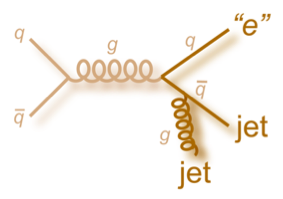
\includegraphics[width=0.4\textwidth]{Figures/QCD_diag.png}
		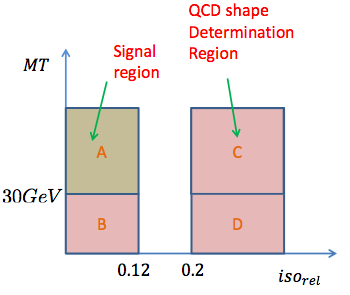
\includegraphics[width=0.45\textwidth]{Figures/QCD_AB.png}		
		%\rule{35em}{0.5pt}
	\caption[QCD diagram and illustration of QCD background determination]{An example of QCD event which looks like signal event (\textit{left}) and illustration of ABCD method used for QCD background determination(\textit{right})}
	\label{fig:QCD}
\end{figure} 

\begin{figure}[htbp]
	\centering
		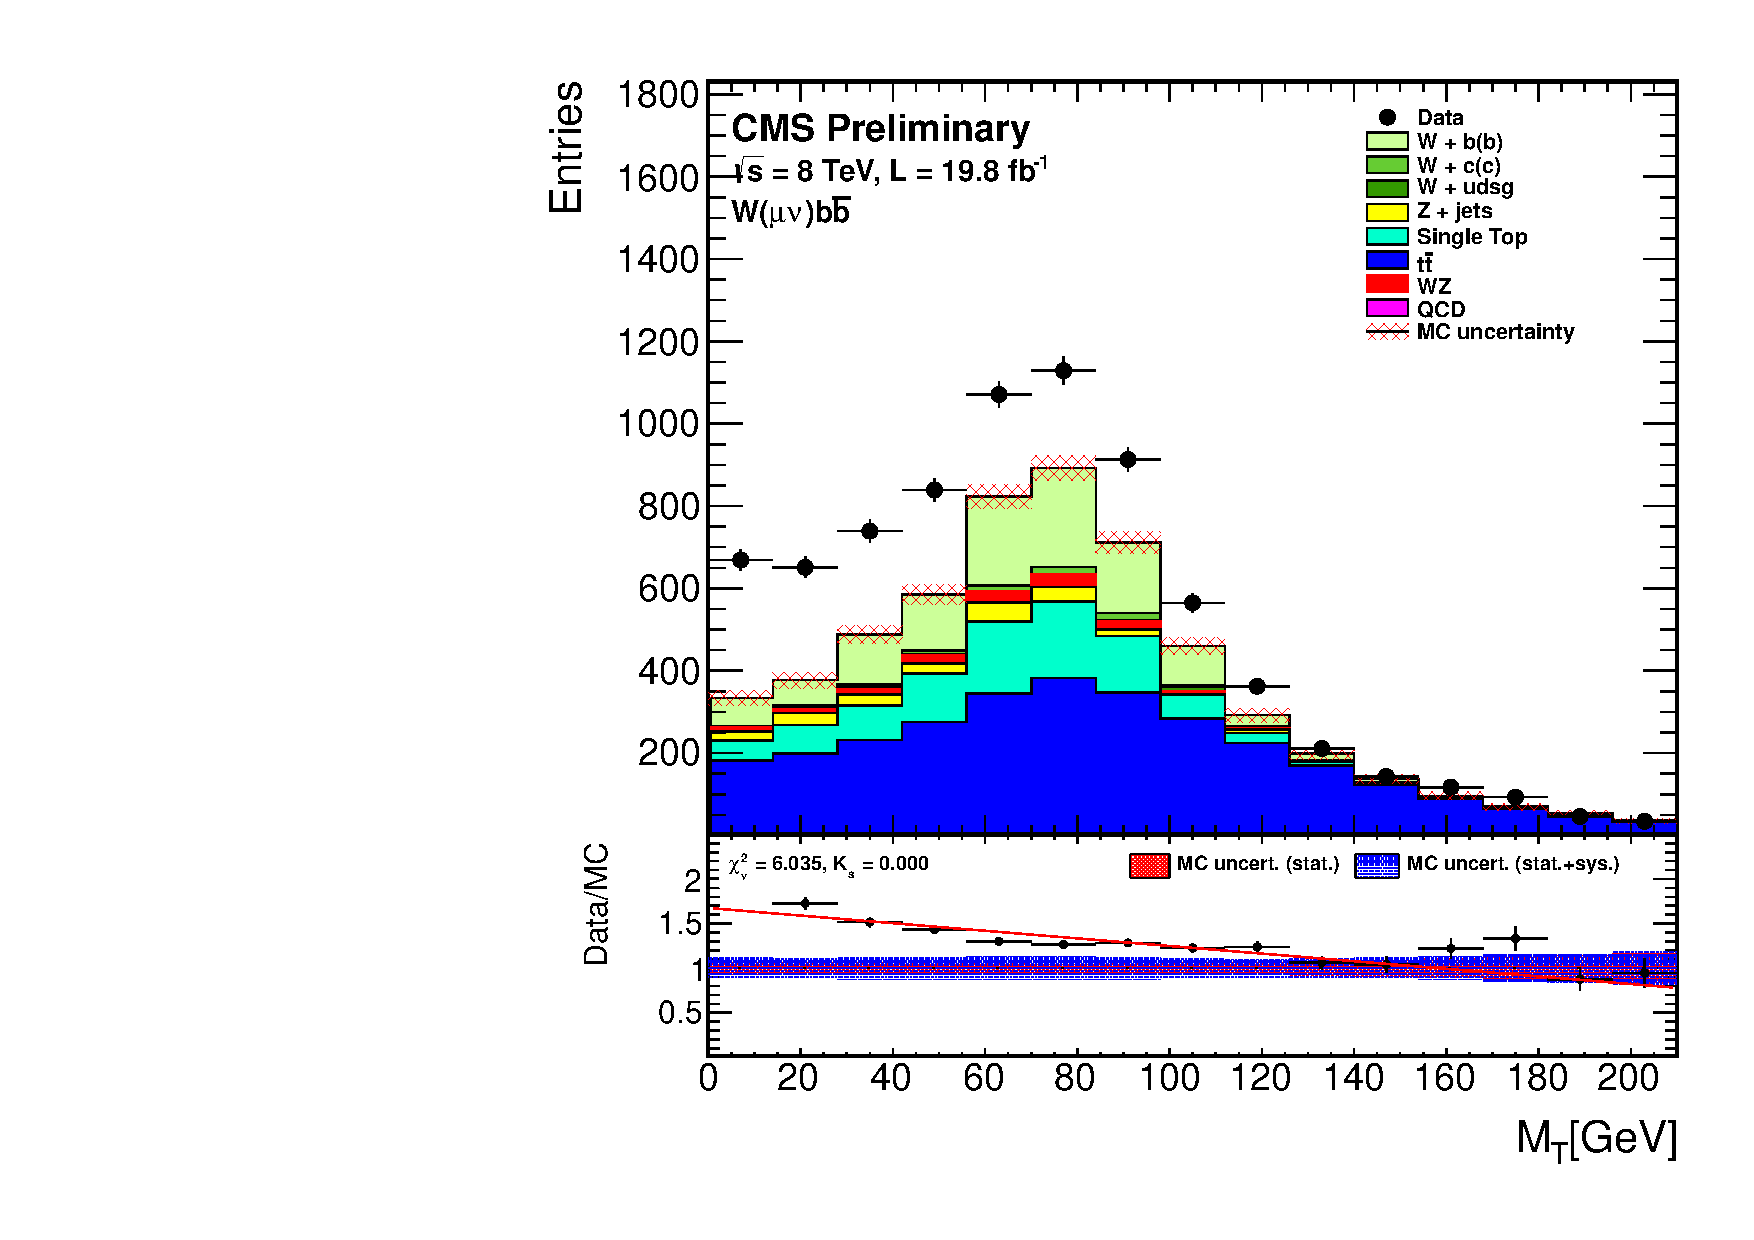
\includegraphics[width=0.48\textwidth]{Figures/VMt_QCD_before.pdf}
		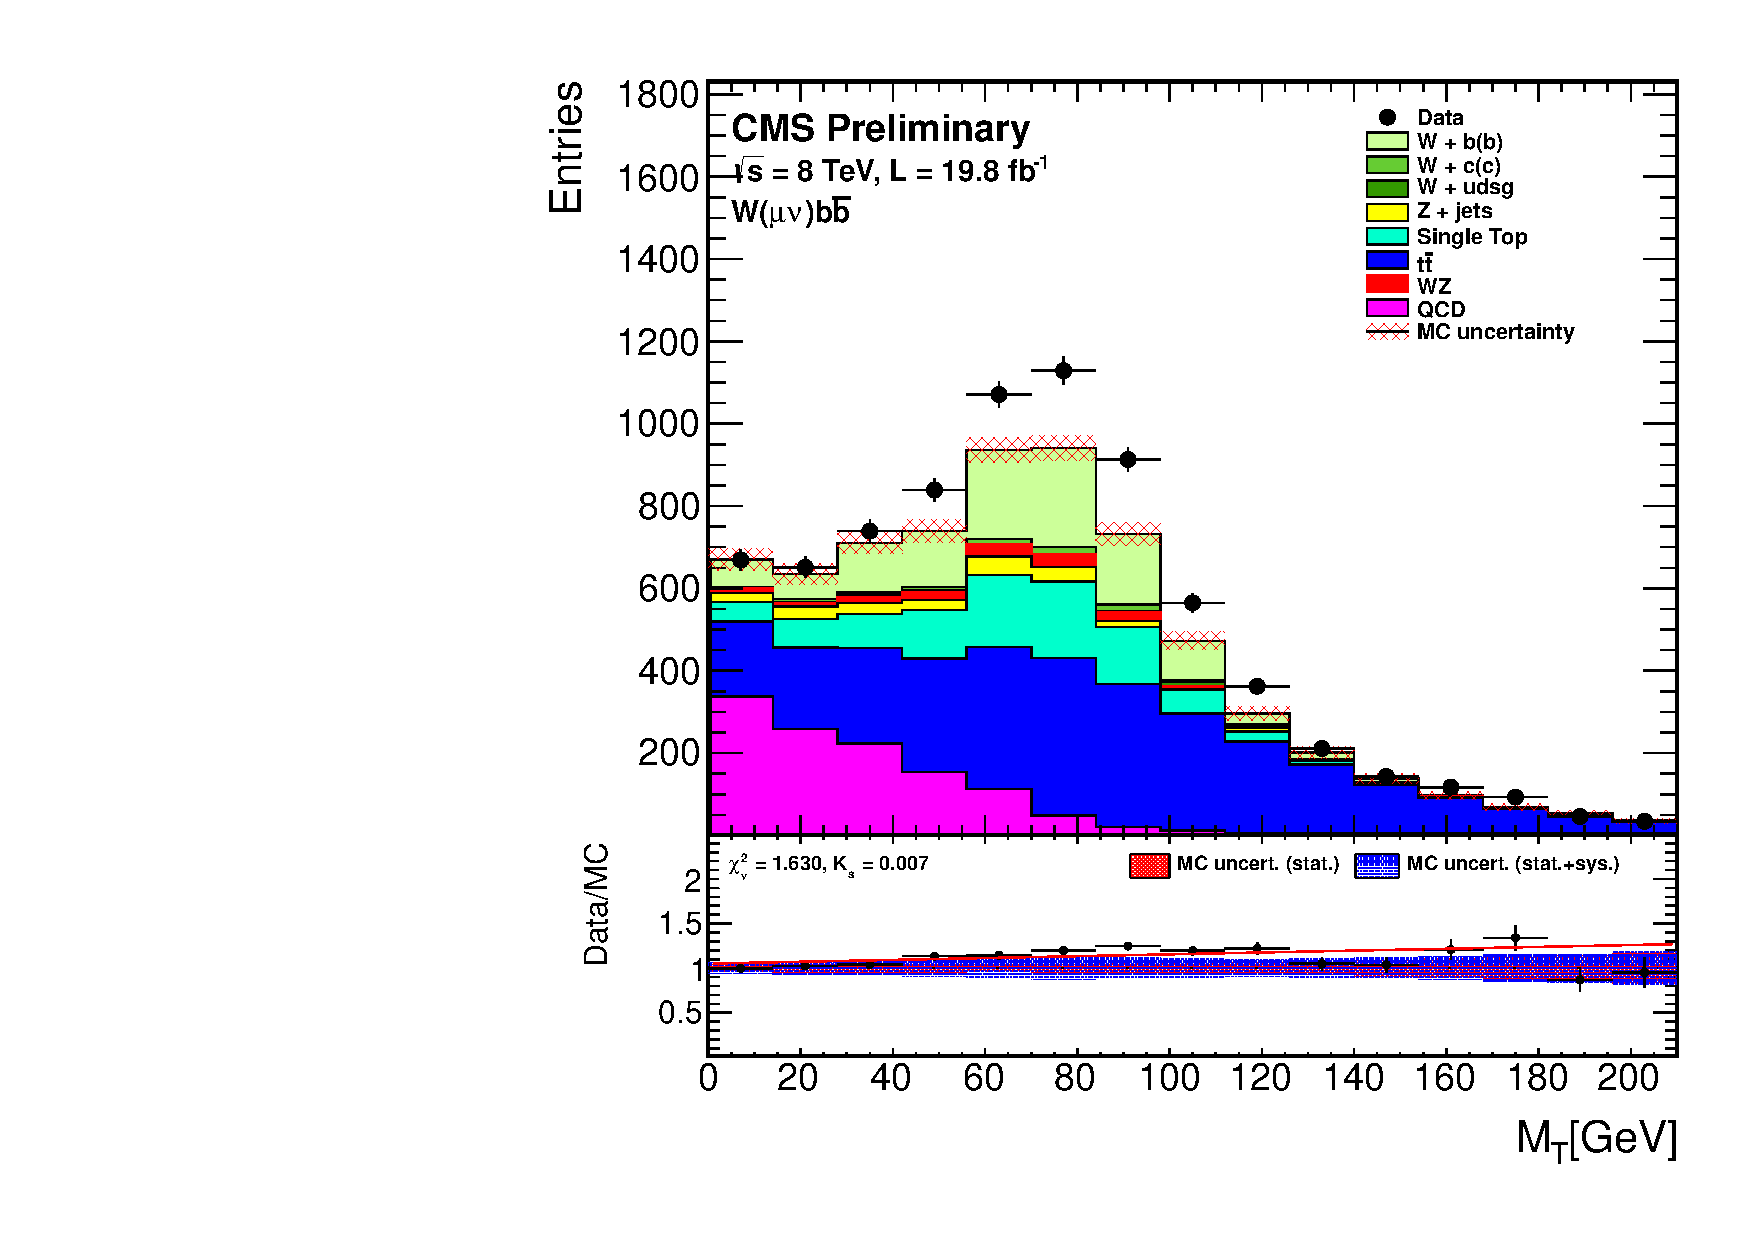
\includegraphics[width=0.48\textwidth]{Figures/VMt_QCD_after.pdf}		
		%\rule{35em}{0.5pt}
	\caption[Transverse mass distribution before and after QCD distribution determination.]{Transverse mass distribution before(\textit{left}) and after QCD background determination(\textit{right}).}
	\label{fig:QCD_dist}
\end{figure} 


\subsection{Other backgrounds}
Other backgrounds include processes with final states that match the final state of the signal. One of such signals is WZ where W decays leptonically and Z decays in a pair of b quarks. Another example is the production of Higgs boson in association with W boson where Higgs also decays to a pair of  quarks. Such backgrounds are called irreducible backgrounds.


%-----------------------------------
%	SECTION 3
%-----------------------------------
\section{Monte-Carlo corrections}
\label{sec:mcSF}

\subsection{Pileup}

In proton-proton collisions at high beam intensities, there is a high probability that multiple interactions could happen. These additional interactions are usually referred to as pileup interactions. The average number of additional interactions during 2012 was 21 with some events going up to 70. With these conditions it is important to be able to recognize the signature from such interactions. Usually pileup originates form low$-p_T$ QCD jets. The identification of pileup jets as well as their removal is described in detail in \cite{CMS:2013wea}. 
\par Simulated events have different distribution for number of pileup interaction with respect to data. This occurs because when generating simulated events, it was difficult to predict the exact pileup distribution in data. Therefore, simulated events to be rewighted to match the distribution in data. The data pile up distribution in the collision period was estimated assuming total proton-proton cross section of 68 mb. For each simulated event, a weight $w_{PU}$ is derived based on the number of pileup events provided by the generator. Figure \ref{fig:N_pu} shows number of pile-up events before and after the rewighting procedure for signal events in the muon channel. The agreement between data and simulation has clearly improved after the procedure. 

\begin{figure}[htbp]
	\centering
		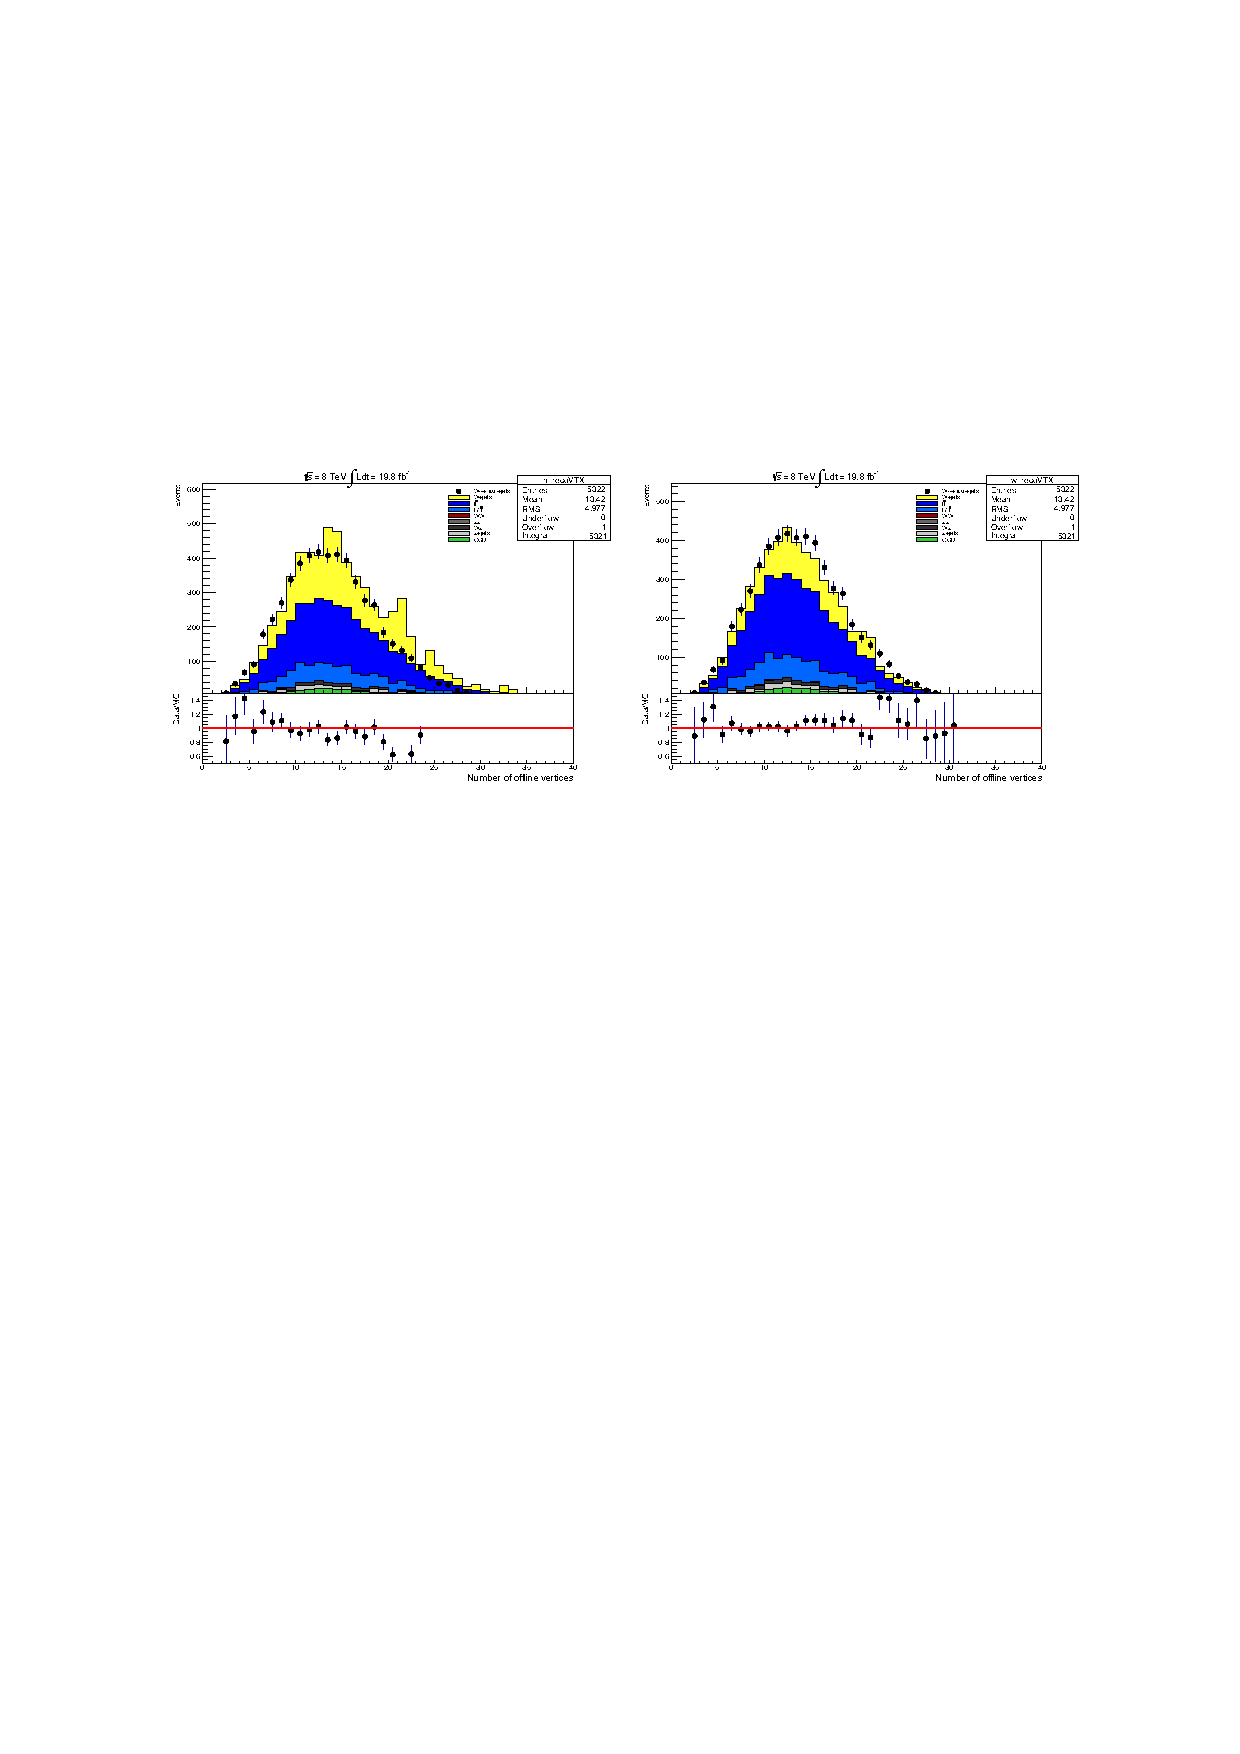
\includegraphics[width=0.9\textwidth]{Figures/NPU_placeholder.pdf}
		%\rule{35em}{0.5pt}
	\caption[Placeholder - PU]{Placeholder - $N_PU$}
	\label{fig:N_pu}
\end{figure} 

\subsection{Lepton efficiency measurement}

Events used for cross section measurement are required to pass certain triggers in order to be selected. However, trigger selection is not 100$\%$ efficient and the selection efficiency has to be measured. The following steps in the analysis like reconstruction and isolation have some inefficiencies as well. Efficiency estimation from simulation shows large systematic errors due to inaccuracy in signal modeling and detector response. This was the main motivation for development of the fully data-driven efficiency estimation called \textit{Tag and probe}. Using well-known mass resonances, such as Z boson mass resonance, a selection criteria is applied to the decay products. \textit{Tag} lepton is the one passing very tight selection cuts with low missidentification probability. The efficiency for certain cuts is than measured by counting \textit{probe} leptons which are leptons passing this looser cut divided by number of all leptons. Probes are selected in such way that the invariant mass of the two leptons falls into the Z mass resonance. The following relation is used for the measurement:
\begin{equation}
\epsilon = \frac{N_{pass}}{N_{pass}+N_{fail}}
\end{equation}   
Final selection contains a number of events where Z boson was not actually produced and which have to be subtracted. Both signal and background contributions are parametrized their relative contributions are estimated using Maximum likelihood fit. For signal events a convolution of Z generator shape with a Gaussian is used to take into account the detector effects, while for background parametrization, a combination of exponential function and polinomial was used.
\par The efficiency was measured as a function of pseudorapidity and transverse momentum of a passing probe. Trigger, identification and isolation criteria were used in electron and muon channels separately. Both data and Monte Carlo efficiencies were measured and their ratio was used as a scale factor for each event in order to match simulated lepton efficiencies to measured data. Muon identification and isolation efficiency measurement for data and MC is shown in figure \ref{fig:eff_IDISO} while trigger efficiency measurement is shown in figure \ref{fig:eff_trig}.

\begin{figure}[htbp]
	\centering
		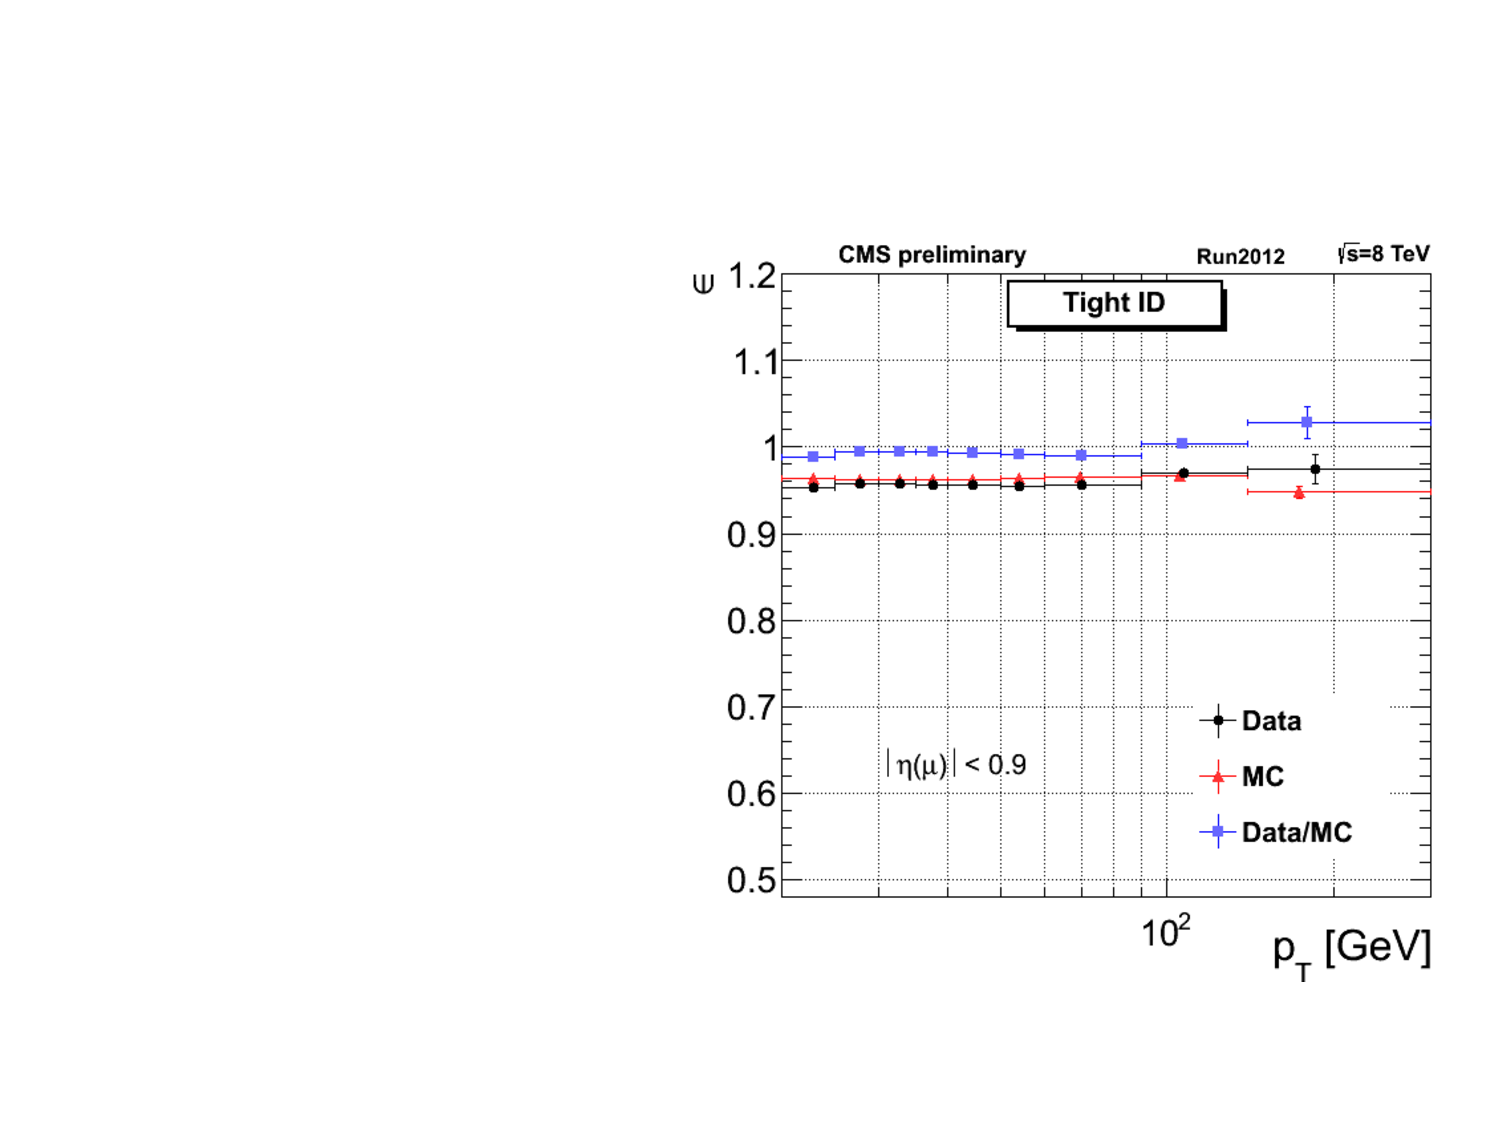
\includegraphics[width=0.49\textwidth]{Figures/ID_eff.pdf}
		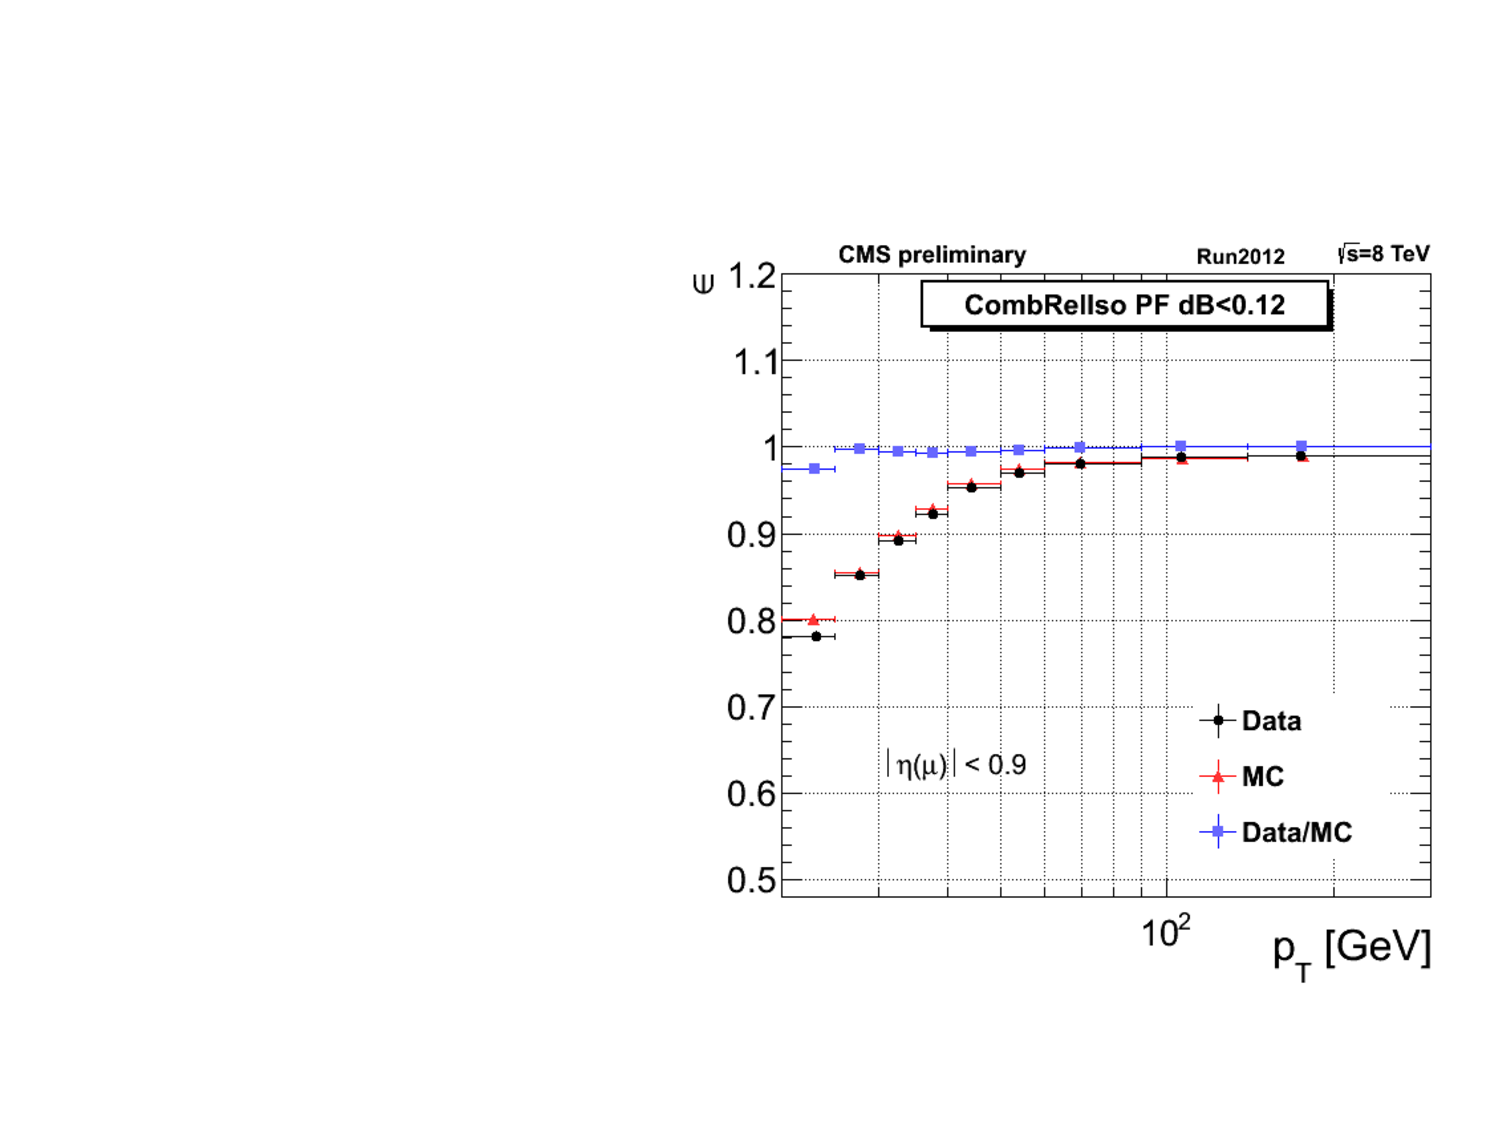
\includegraphics[width=0.49\textwidth]{Figures/ISO_eff.pdf}
		%\rule{35em}{0.5pt}
	\caption[Muon identification and isolation efficiencies using \textit{tag and probe} method.]{Muon identification and isolation efficiencies as a function of a probe $p_T$ using \textit{tag and probe} method. The measurement shown here is for barrel part of the detector$(\eta<0.9)$, but similar measurements were performed for the region between barrel and endcap$(0.9<\eta<1.2)$ and endcap $(1.2<\eta<2.1)$ separately.}
	\label{fig:eff_IDISO}
\end{figure}

\begin{figure}[htbp]
	\centering
		\includegraphics[width=0.5\textwidth]{Figures/trig_eff.pdf}
		%\rule{35em}{0.5pt}
	\caption[Muon trigger efficiency using \textit{tag and probe} method.]{Muon trigger efficiency for $\mathrm{HLT\_IsoMu24}$ using \textit{tag and probe} method of barrel part of the detector $(\eta<0.9)$.}
	\label{fig:eff_trig}
\end{figure}  



\subsection{\textit{b-tagging} scale factors}
